\documentclass[11pt,a4paper]{article}

\usepackage[T1]{fontenc}
\usepackage[utf8]{inputenc}
\usepackage{mathptmx}
\usepackage{courier}
\usepackage[margin=2.5cm]{geometry}
\usepackage{amsmath}
\usepackage{booktabs}
\usepackage{graphicx}
\usepackage{xcolor}
\usepackage[numbers,sort&compress]{natbib}
\usepackage{xurl}
\usepackage[hidelinks]{hyperref}
\hypersetup{pdftitle={Right Once, Wrong Next Time: Repeated-Trial Reliability of Small Local Models on Roman Urdu Clinic Tool Calls},pdfauthor={Muzammal Hussain}}
\usepackage{caption}
\captionsetup{font=small,labelfont=bf}

\newcommand{\code}[1]{\texttt{#1}}
\newcommand{\passk}[1]{pass$^{#1}$}
\setlength{\emergencystretch}{3em}

\title{\textbf{Right Once, Wrong Next Time: Repeated-Trial Reliability of\\Small Local Models on Roman Urdu Clinic Tool Calls}}
\author{Muzammal Hussain\\
\small Independent researcher, Glasgow, United Kingdom\\
\small \href{mailto:muzammal@masmatixinnovations.co.uk}{muzammal@masmatixinnovations.co.uk}\\
\small ORCID: \href{https://orcid.org/0009-0001-2570-5686}{0009-0001-2570-5686}}
\date{\small November 2026}

\begin{document}
\maketitle

\begin{abstract}
\noindent
Tool-use evaluations usually score one attempt per task, but an agent that books the right appointment four times
out of five is not safe to leave unattended. We measure \passk{k}, the probability that all $k$ attempts at the same
task are correct, for two small open-weight models run locally (\code{llama3.1:8b} and \code{qwen2.5:3b}) on eight
physiotherapy-clinic tool calls requested in English and in Roman Urdu, the Latin-script Urdu that many people in
Pakistan and its diaspora type. Each task was attempted five times in two ways: with five wordings of the same
request at temperature 0, and with one wording sampled five times at temperature 0.7 (320 calls). In English,
\passk{5} was 87.5\% for \code{llama3.1:8b} and 75.0\% for \code{qwen2.5:3b} in both conditions. In Roman Urdu it
fell to 12.5--37.5\%, and single attempts hid the gap: with five wordings, \code{qwen2.5:3b} got 62.5\% of single
attempts right but only 12.5\% of tasks right every time. Rewording made Roman Urdu tasks intermittently wrong;
sampling made them systematically wrong, with up to half of the tasks failing in all five samples, so a retry would
not have helped. The failures concentrated in values that need interpretation rather than copying: times written as
words (\emph{dhai baje}, half past two), number words, a refund amount, a cancellation reason and a city. 67 of the 73
failed calls (91.8\%) were valid against the tool schema, and in an earlier pilot a validator-feedback loop never
triggered while a quarter of calls carried wrong values. For clinic agents in code-mixed languages, schema
validation is not a safety check; repeated-trial evaluation and read-back confirmation of interpreted values are
needed. All prompts, replies and analysis code are public.
\end{abstract}

\noindent\textbf{Keywords:} LLM agents; tool calling; pass$^k$; reliability; Roman Urdu; code-mixed language; local language models; clinical software

\section{Introduction}

An agent acts through tool calls: it books an appointment, records a pulse or refunds a payment by filling a
structured argument list. Benchmarks usually report how often the first attempt is correct. For deployment the more
useful question is whether the agent is correct \emph{every} time it meets the same request, because a clinic runs
the same kinds of request hundreds of times a week. $\tau$-bench introduced \passk{k}, the probability that all $k$
independent attempts at a task succeed, and found that even state-of-the-art function-calling agents succeeded on fewer than half of
the tasks and that \passk{8} fell below 25\% in the retail domain~\cite{yao2024tau}. That study used English and large hosted models, and its
repeated attempts varied both the simulated user's wording and the model's sampling.

Small clinics, especially in Pakistan and among its diaspora, have two further constraints. Patient data should stay
on local hardware, which favours models of a few billion parameters. And staff often write in Roman Urdu: Urdu in
the Latin alphabet with English terms mixed in and no fixed spelling, a setting in which language technology is
scarce~\cite{butt2025romanir,butt2025transliteration} and code-mixed text is known to be hard for NLP
systems~\cite{khanuja2020gluecos}. In earlier work we found that Roman Urdu input reduced the accuracy of small local
ReAct agents on clinic questions by up to 35 points~\cite{hussain2026romanurdu}. Here we ask the narrower question
of single tool calls:

\begin{enumerate}
  \item How repeatable are small local models' clinic tool calls in English and in Roman Urdu, measured by
  \passk{k}?
  \item Is the variation driven by how the request is worded or by random sampling?
  \item Which arguments fail, and would a schema validator catch them?
\end{enumerate}

\section{Method}

\paragraph{Tasks.} Eight clinic tools, each with a JSON schema and a ground-truth argument list: book an
appointment, record vital signs, record a pain score, set a reminder, refund a payment, cancel an appointment,
search patients, and log an exercise. Each request was written in English and in Roman Urdu (Table~\ref{tab:examples})
and deliberately includes values given in words: ``half past two in the afternoon''/\emph{dopahar dhai baje},
``seventy-two''/\emph{bahattar}, ``forty-five pounds fifty''/\emph{paintalees pound pachaas pence}.

\begin{table}[t]
\centering
\small
\caption{Examples of the requests and the values the tool call must contain.}
\label{tab:examples}
\begin{tabular}{p{2.1cm}p{5.6cm}p{4.2cm}}
\toprule
Tool & Roman Urdu request & Required values \\
\midrule
Book appointment & \emph{Patient number 4417 ki appointment 3 November 2026 ko dopahar dhai baje book karo. Urgent nahi hai.} & time 14:30, urgent false \\
Record vitals & \emph{Patient 2093 ke vitals save karo: BP 128/84, pulse bahattar.} & 128, 84, pulse 72 \\
Refund & \emph{Invoice INV-1029 ke paintalees pound pachaas pence wapas kar do.} & amount 45.50, GBP \\
Cancel & \emph{Appointment 55821 cancel karo kyunke physio beemar hai, aur patient ko bata do.} & reason clinician\_unavailable, notify true \\
Search & \emph{Glasgow mein Akhtar surname wale zyada se zyada paanch patients dhoondo.} & last name Akhtar, city Glasgow, 5 \\
\bottomrule
\end{tabular}
\end{table}

\paragraph{Two sources of variation.} Each task was attempted five times per language in two conditions.
\emph{Wording}: the original request and four rewordings with the same meaning, at temperature 0 and seed 42; the
Roman Urdu rewordings use the spelling variety people actually type (\emph{kr/kar}, \emph{dopehar/dopahar},
\emph{nai/nahi}). \emph{Sampling}: the original wording at temperature 0.7 with seeds 1--5. The grid is
2 models $\times$ 8 tasks $\times$ 2 languages $\times$ 2 conditions $\times$ 5 attempts = 320 calls.

\paragraph{Models and scoring.} \code{qwen2.5:3b}~\cite{qwen2025qwen25} and \code{llama3.1:8b}~\cite{grattafiori2024llama3}
ran through Ollama on a MacBook (Apple M4, 16\,GB) with at most 256 output tokens; a call that timed out after 120\,s
was retried once (none did in the final run). An attempt passes if the reply is valid against the tool schema and
every value matches the ground truth after normalising case and punctuation. We report \passk{k} with the unbiased
estimator of $\tau$-bench, $\binom{c}{k}/\binom{n}{k}$ averaged over tasks, with $n=5$ attempts and $c$ passes, and
95\% percentile bootstrap intervals over the eight tasks (2,000 resamples)~\cite{efron1993bootstrap}. We also count
tasks that always, sometimes or never pass, and the number of distinct outputs per task.

\paragraph{Validator pilot.} Before this study we ran each of the eight tasks once per language with
\code{qwen2.5:3b} at temperature 0 inside a self-correction loop: if a schema validator found problems, they were
sent back to the model for up to two retries, without the expected values.

\section{Results}

\subsection{English is repeatable, Roman Urdu is not}

Table~\ref{tab:passk} and Figure~\ref{fig:passk} give \passk{k} for $k=1$ to 5. In English, both models were mostly
repeatable: \passk{5} was 87.5\% for \code{llama3.1:8b} (7 of 8 tasks right in every attempt) and 75.0\% for
\code{qwen2.5:3b}, identical across the two conditions. In Roman Urdu \passk{5} fell to 37.5\% for
\code{llama3.1:8b} and to 12.5\% (wording) and 25.0\% (sampling) for \code{qwen2.5:3b}. Single attempts understated
the problem most when the wording varied: \code{llama3.1:8b} went from 80.0\% at $k=1$ to 37.5\% at $k=5$, and
\code{qwen2.5:3b} from 62.5\% to 12.5\%. With eight tasks the intervals are wide; the gap between languages is
clear, but differences between models and conditions are not.

\begin{table}[t]
\centering
\small
\caption{\passk{1} and \passk{5} (\%) with 95\% bootstrap intervals over the 8 tasks, task outcome counts and the mean
number of distinct outputs per task.}
\label{tab:passk}
\setlength{\tabcolsep}{4pt}
\footnotesize
\begin{tabular}{llllllc}
\toprule
Model & Language & Condition & \passk{1} & \passk{5} & Always / some / never & Distinct \\
\midrule
\code{llama3.1:8b} & English & wording  & 97.5 [92.5, 100] & 87.5 [62.5, 100] & 7 / 1 / 0 & 1.12 \\
\code{llama3.1:8b} & English & sampling & 97.5 [92.5, 100] & 87.5 [62.5, 100] & 7 / 1 / 0 & 1.12 \\
\code{llama3.1:8b} & Roman Urdu & wording  & 80.0 [67.5, 92.5] & 37.5 [0.0, 75.0] & 3 / 5 / 0 & 1.88 \\
\code{llama3.1:8b} & Roman Urdu & sampling & 47.5 [12.5, 82.5] & 37.5 [12.5, 75.0] & 3 / 1 / 4 & 1.62 \\
\code{qwen2.5:3b} & English & wording  & 95.0 [87.5, 100] & 75.0 [37.5, 100] & 6 / 2 / 0 & 1.25 \\
\code{qwen2.5:3b} & English & sampling & 85.0 [60.0, 100] & 75.0 [37.5, 100] & 6 / 1 / 1 & 1.12 \\
\code{qwen2.5:3b} & Roman Urdu & wording  & 62.5 [47.5, 77.5] & 12.5 [0.0, 37.5] & 1 / 7 / 0 & 2.50 \\
\code{qwen2.5:3b} & Roman Urdu & sampling & 52.5 [22.5, 80.0] & 25.0 [0.0, 62.5] & 2 / 3 / 3 & 1.62 \\
\bottomrule
\end{tabular}
\end{table}

\begin{figure}[t]
  \centering
  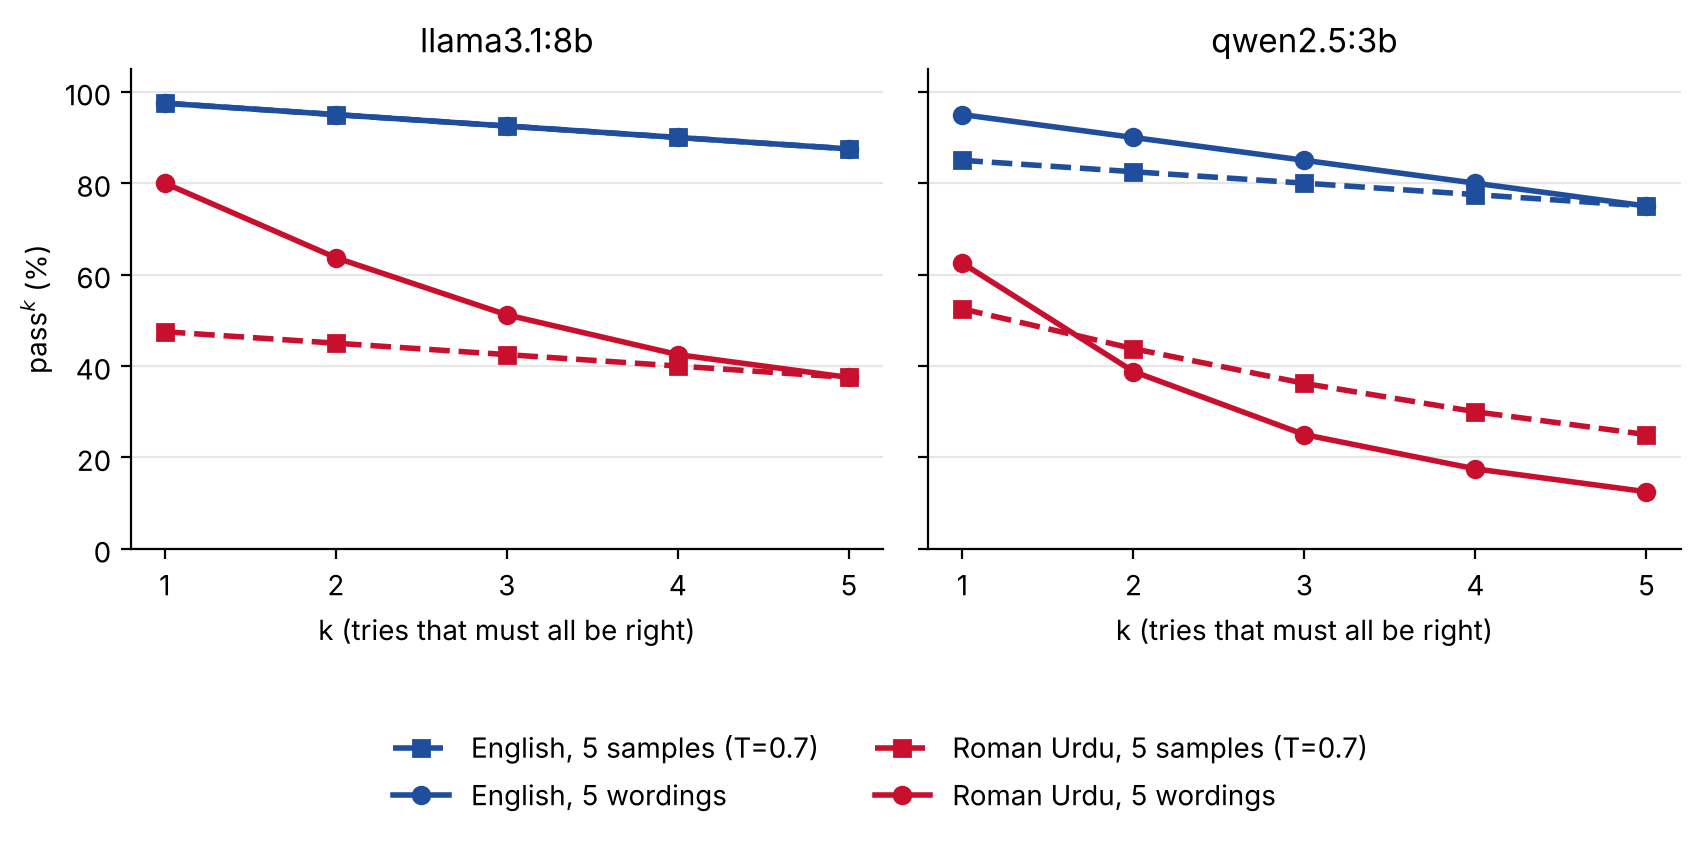
\includegraphics[width=\linewidth]{figures/fig_passk.png}
  \caption{\passk{k} for $k=1$ to 5. Blue: English; red: Roman Urdu. Solid: five wordings at temperature 0; dashed:
  one wording sampled five times at temperature 0.7.}
  \label{fig:passk}
\end{figure}

\subsection{Wording and sampling fail differently}

The two conditions produced different kinds of failure in Roman Urdu. Rewording made tasks \emph{intermittently}
wrong: for \code{llama3.1:8b} 5 of 8 tasks and for \code{qwen2.5:3b} 7 of 8 were right in some wordings and wrong in
others, and \code{qwen2.5:3b} produced 2.5 distinct outputs per task on average. Sampling the original wording made
failures \emph{systematic}: \code{llama3.1:8b} got 4 of the 8 Roman Urdu tasks wrong in all five samples (the
appointment time, the pulse, the refund amount and the cancellation reason), and \code{qwen2.5:3b} got 3 wrong in
all five. For those tasks, retrying with a new random seed would not have helped; the model consistently read the
request the wrong way.

\subsection{Which values break}

Of the 320 calls, 73 failed: 63 in Roman Urdu and 10 in English (Figure~\ref{fig:fields}). The failures were in
values that require interpretation rather than copying. The time \emph{dopahar dhai baje} (14:30) was written as 14:00
(7 calls) or 13:00 (6), so ``\emph{dhai}'' (two and a half) lost its half. The refund of 45.50 became 45.0 (6 calls),
and in 4 calls 100, a number that does not appear in the request. The pulse \emph{bahattar} (72) became 100 in 4
calls. ``Physio \emph{beemar} hai'' (the physiotherapist is ill) was mapped to the generic reason \code{other} instead
of \code{clinician\_unavailable} in 6 calls. The city in ``\emph{Glasgow mein}'' (in Glasgow) was left empty in 7
calls. The exercise log, where every value is a plain number or a word copied from the request, was right in all 40
attempts in both languages. In English the errors were mostly the same refund fraction (6 calls dropped the 50 pence).

\begin{figure}[t]
  \centering
  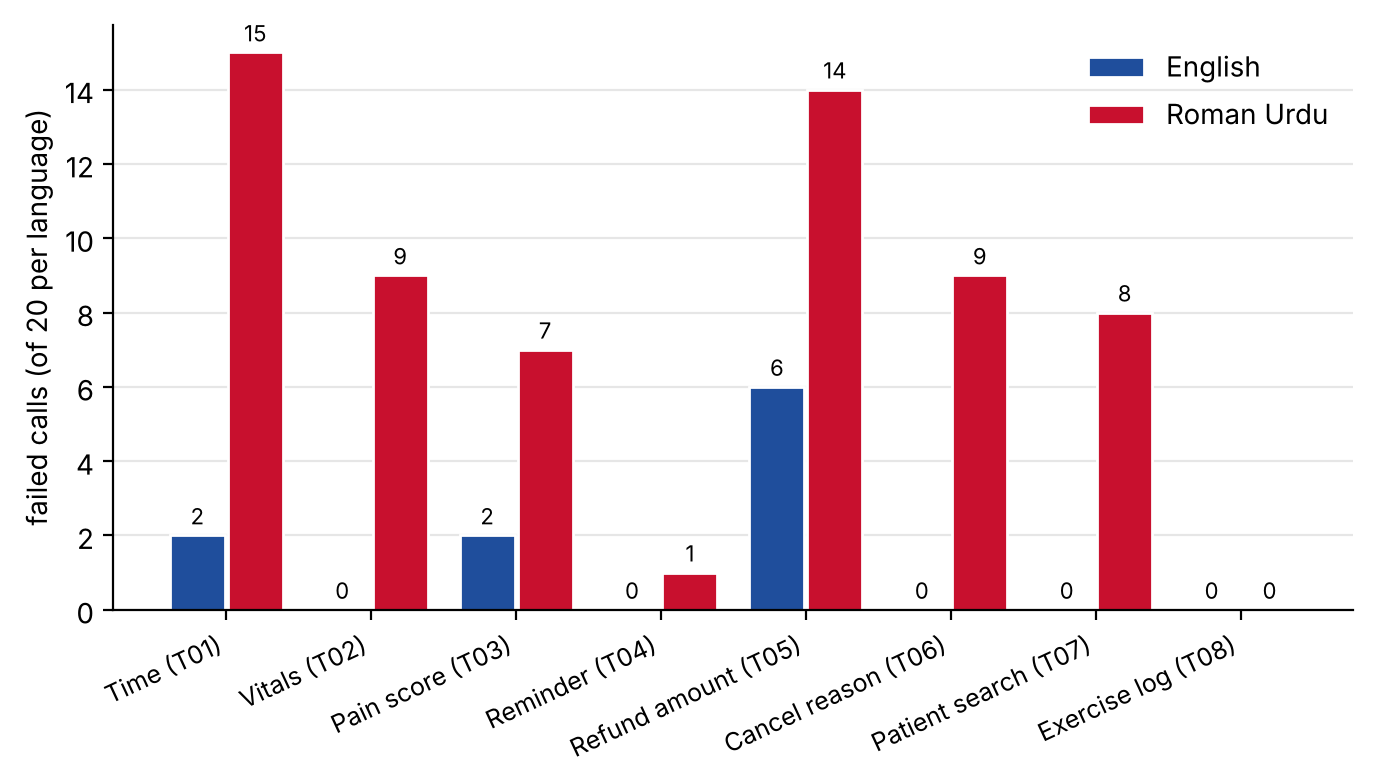
\includegraphics[width=0.8\linewidth]{figures/fig_fail_tasks.png}
  \caption{Failed calls per task and language, out of 20 per task and language (2 models $\times$ 2 conditions
  $\times$ 5 attempts).}
  \label{fig:fields}
\end{figure}

\subsection{A schema validator would not have caught them}

67 of the 73 failed calls (91.8\%) were valid against the tool schema: correct keys, types and formats, with a wrong
value. An empty city is still a string; 14:00 is a valid time. The earlier validator pilot shows the same from the
other side: all 16 calls of \code{qwen2.5:3b} passed the validator at the first attempt, so the self-correction loop
never ran, yet 4 of them (3 in Roman Urdu) carried a wrong value, including the invented refund of 100. Output
formatting was a minor issue by comparison: 150 of the 320 replies wrapped the JSON in code fences despite being
told not to, but they could still be parsed.

\section{Discussion}

\paragraph{Score more than one attempt.} For English the single-attempt score was a fair guide to repeatability.
For Roman Urdu it was not: a model that is right on 80\% of single attempts can be right on every attempt for only
37.5\% of tasks. Evaluations of agents for code-mixed or low-resource languages should report \passk{k} or the
number of tasks that are always right, not only accuracy.

\paragraph{Vary the wording, not only the seed.} Sampling and rewording expose different risks. Rewording shows
that the same meaning in a different spelling or phrasing can flip a call; sampling shows that some requests are
read wrongly every time. A test set built from one wording per task and repeated seeds would miss the first kind;
one attempt per wording would miss the second.

\paragraph{Validate meaning, not only shape.} Almost all failures were schema-valid. Stricter schemas help with
some (no empty strings, a plausible range for a pulse), but an appointment at 14:00 instead of 14:30 is only caught by
comparing the call with what the user meant. For a clinic tool, a read-back step (``Book 4417 on 3 November at
14:30, is that right?'') is the simplest safeguard for interpreted values such as times, amounts and doses.

\paragraph{Number words are the weak point.} The values that broke most were numbers and times written as words in
Roman Urdu, together with the free-text reason and city. Normalising number words to digits before the model sees
them is a cheap intervention that this study suggests but does not test.

\section{Limitations}

Eight tasks is a pilot: one task is 12.5 percentage points, and the bootstrap intervals are wide. The requests and
rewordings were written by the author and are not a sample of real clinic messages; other Roman Urdu spellings may
behave differently. Each call is a single turn, whereas $\tau$-bench scores full conversations. Scoring is exact match
after light normalisation, so a correct paraphrase of a free-text field counts as wrong. Ollama seeds make runs
repeatable on one machine but not necessarily across versions or hardware. The validator pilot used one model and
16 calls. No clinician reviewed the tasks, and no patient data were used.

\section{Conclusion}

Two small local models made clinic tool calls in English that were mostly repeatable, but in Roman Urdu the same
tasks were right every time for only one in eight to three in eight tasks, depending on the model and the source of
variation. The failures were schema-valid errors in interpreted values, especially numbers and times written as
words. Before small local agents act on Roman Urdu requests, they should be evaluated over repeated attempts and
rewordings, and interpreted values should be read back to the user before the call runs.

\section*{Code and data availability}

The tasks, the rewordings, all 320 raw replies, the validator pilot and the analysis code are in the folders
\code{tool-call-consistency} and \code{tool-call-self-correction} of the author's research log, archived at
\url{https://doi.org/10.5281/zenodo.24230498} and developed at \url{https://github.com/MHKhan50/agentic-ai-research-log}.
All requests are invented; no patient data were used.

\bibliographystyle{unsrtnat}
\bibliography{references}

\end{document}
